\documentclass{standalone}

% In your preamble:
\usepackage{tikz}
\usetikzlibrary{calc}

\tikzset{
  axis length/.store in=\AxisLen,
  plane length/.store in=\PlaneLen,
  x foreshorten/.store in=\ForeshortenX,
  x angle/.store in=\AngleX,
  axis length=3,
  plane length=2.4,
  x foreshorten=0.7,
  x angle=-135
}

\begin{document}

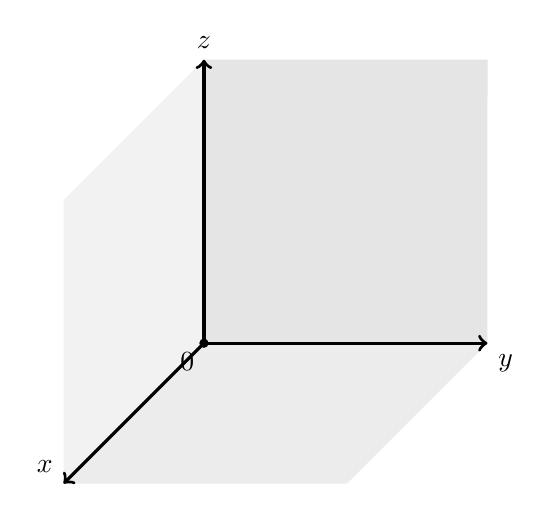
\begin{tikzpicture}[scale=1.2, line cap=round, line join=round]

  % Basis directions in the page (a projection of R^3):
  % y: to the right
  % z: straight up
  % x: 135 degrees from y (i.e., up-left)
  \coordinate (O) at (0,0);
  \coordinate (Y) at (\AxisLen,0);
  \coordinate (Z) at (0,\AxisLen);
  \coordinate (X) at ({\ForeshortenX*\AxisLen*cos(\AngleX)},{\ForeshortenX*\AxisLen*sin(\AngleX)});

  % Useful derived points
  \coordinate (XY) at ($(X)+(Y)$);
  \coordinate (XZ) at ($(X)+(Z)$);
  \coordinate (YZ) at ($(Y)+(Z)$);

  % Lightly shade the three coordinate planes in the positive orthant
  \fill[gray!15] (O) -- (X) -- (XY) -- (Y) -- cycle; % xy-plane
  \fill[gray!10] (O) -- (X) -- (XZ) -- (Z) -- cycle; % xz-plane
  \fill[gray!20] (O) -- (Y) -- (YZ) -- (Z) -- cycle; % yz-plane

  % Draw axes
  \draw[->, very thick] (O) -- (X) node[above left] {$x$};
  \draw[->, very thick] (O) -- (Y) node[below right] {$y$};
  \draw[->, very thick] (O) -- (Z) node[above] {$z$};

  % Optional: mark the origin
  \fill (O) circle (1.4pt) node[below left] {$0$};
\end{tikzpicture}



% Preamble:
% \usepackage{tikz}
% \usetikzlibrary{calc}

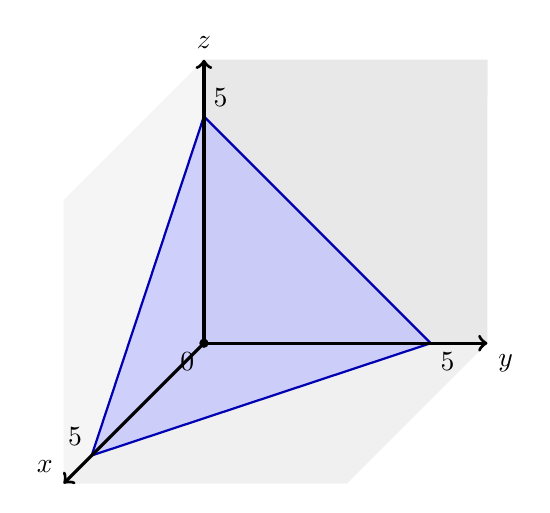
\begin{tikzpicture}[scale=1.2, line cap=round, line join=round]

  % Origin
  \coordinate (O) at (0,0);

  % Axes directions (projection)
  \coordinate (Y) at (\AxisLen,0);                 % y axis
  \coordinate (Z) at (0,\AxisLen);                 % z axis
  \coordinate (X) at ({\ForeshortenX*\AxisLen*cos(\AngleX)},{\ForeshortenX*\AxisLen*sin(\AngleX)}); % x axis

  % Plane intercepts (scaled)
  \coordinate (PX) at ({\ForeshortenX*\PlaneLen*cos(\AngleX)},{\ForeshortenX*\PlaneLen*sin(\AngleX)}); % (5,0,0)
  \coordinate (PY) at (\PlaneLen,0);                        % (0,5,0)
  \coordinate (PZ) at (0,\PlaneLen);                        % (0,5,0)

  % Derived corners
  \coordinate (XY) at ($(X)+(Y)$);
  \coordinate (XZ) at ($(X)+(Z)$);
  \coordinate (YZ) at ($(Y)+(Z)$);

  % Coordinate planes (positive orthant)
  \fill[gray!12] (O) -- (X) -- (XY) -- (Y) -- cycle; % xy
  \fill[gray!8]  (O) -- (X) -- (XZ) -- (Z) -- cycle; % xz
  \fill[gray!18] (O) -- (Y) -- (YZ) -- (Z) -- cycle; % yz

  % Plane a+b+c=5 (simplex face)
  \fill[blue!25, opacity=0.7]
    (PX) -- (PY) -- (PZ) -- cycle;

  % Plane edges
  \draw[thick, blue!70!black]
    (PX) -- (PY) -- (PZ) -- cycle;

  % Axes
  \draw[->, very thick] (O) -- (X) node[above left] {$x$};
  \draw[->, very thick] (O) -- (Y) node[below right] {$y$};
  \draw[->, very thick] (O) -- (Z) node[above] {$z$};

  % Labels for intercepts
  \node[above left]  at (PX) {$5$};
  \node[below right] at (PY) {$5$};
  \node[above right] at (PZ) {$5$};

  % Origin
  \fill (O) circle (1.4pt) node[below left] {$0$};

\end{tikzpicture}

% Preamble:
% \usepackage{tikz}
% \usetikzlibrary{calc}

% Preamble:
% \usepackage{tikz}
% \usetikzlibrary{calc}

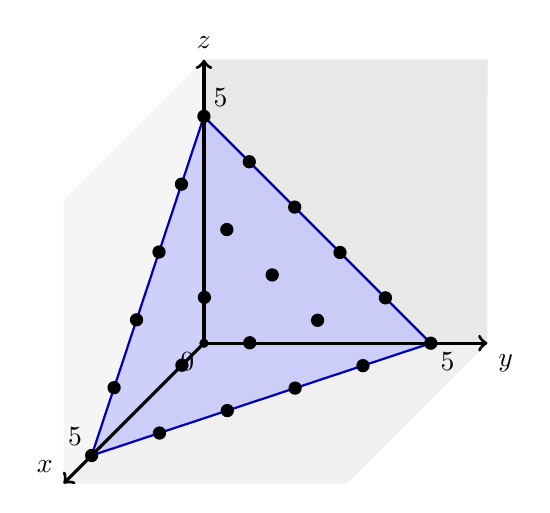
\begin{tikzpicture}[scale=1.2, line cap=round, line join=round]

  \coordinate (O) at (0,0);

  \coordinate (Y) at (\AxisLen,0);
  \coordinate (Z) at (0,\AxisLen);
  \coordinate (X) at ({\ForeshortenX*\AxisLen*cos(\AngleX)},{\ForeshortenX*\AxisLen*sin(\AngleX)});

  \coordinate (PX) at ({\ForeshortenX*\PlaneLen*cos(\AngleX)},{\ForeshortenX*\PlaneLen*sin(\AngleX)});
  \coordinate (PY) at (\PlaneLen,0);
  \coordinate (PZ) at (0,\PlaneLen);

  \coordinate (XY) at ($(X)+(Y)$);
  \coordinate (XZ) at ($(X)+(Z)$);
  \coordinate (YZ) at ($(Y)+(Z)$);

  % coordinate planes
  \fill[gray!12] (O) -- (X) -- (XY) -- (Y) -- cycle;
  \fill[gray!8]  (O) -- (X) -- (XZ) -- (Z) -- cycle;
  \fill[gray!18] (O) -- (Y) -- (YZ) -- (Z) -- cycle;

  % plane a+b+c=5
  \fill[blue!25, opacity=0.7] (PX) -- (PY) -- (PZ) -- cycle;
  \draw[thick, blue!70!black] (PX) -- (PY) -- (PZ) -- cycle;

  % axes
  \draw[->, very thick] (O) -- (X) node[above left] {$x$};
  \draw[->, very thick] (O) -- (Y) node[below right] {$y$};
  \draw[->, very thick] (O) -- (Z) node[above] {$z$};

  \node[above left]  at (PX) {$5$};
  \node[below right] at (PY) {$5$};
  \node[above right] at (PZ) {$5$};
  \fill (O) circle (1.4pt) node[below left] {$0$};

  % ---- lattice points (a,b,c) with a+b+c=5 ----
  \foreach \a in {0,...,5} {
    \foreach \b in {0,...,5} {
      \pgfmathtruncatemacro{\c}{5-\a-\b}
      \ifnum\c<0\relax
      \else
        % weights as decimals
        \pgfmathsetmacro{\wa}{\a/5}
        \pgfmathsetmacro{\wb}{\b/5}
        \pgfmathsetmacro{\wc}{\c/5}

        \coordinate (P) at ($ \wa*(PX) + \wb*(PY) + \wc*(PZ) $);
        \fill (P) circle (2pt);
      \fi
    }
  }

  % Optional: label an example point
  % \coordinate (P410) at ($ 0.8*(PX) + 0.2*(PY) + 0*(PZ) $);
  % \node[font=\small, left] at (P410) {$(4,1,0)$};

\end{tikzpicture}

% Preamble:
% \usepackage{tikz}
% \usetikzlibrary{calc}

% Preamble:
% \usepackage{tikz}
% \usetikzlibrary{calc}

% Preamble:
% \usepackage{tikz}
% \usetikzlibrary{calc}

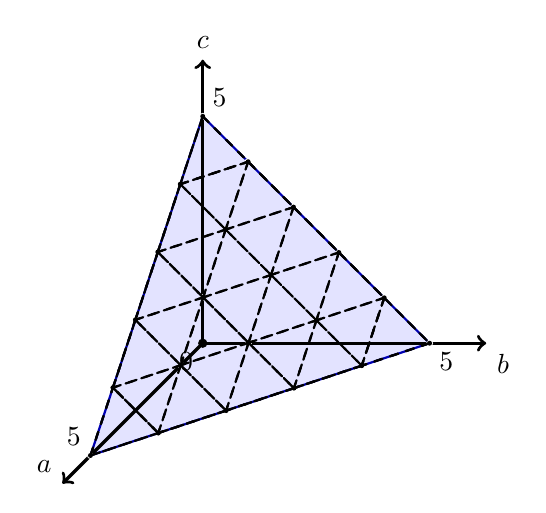
\begin{tikzpicture}[scale=1.2, line cap=round, line join=round]
  % numeric knobs (safe for TikZ math)
  \pgfmathsetmacro{\AxisLen}{3}
  \pgfmathsetmacro{\PlaneLen}{2.4}
  \pgfmathsetmacro{\ForeshortenX}{0.7}
  \pgfmathsetmacro{\N}{5} % plane: a+b+c = 5

  \coordinate (O) at (0,0);

  % projected axes directions
  \coordinate (Y) at (\AxisLen,0);
  \coordinate (Z) at (0,\AxisLen);
  \coordinate (X) at ({\ForeshortenX*\AxisLen*cos(\AngleX)},{\ForeshortenX*\AxisLen*sin(\AngleX)});

  % plane intercepts: (5,0,0), (0,5,0), (0,0,5) (drawn to length PlaneLen)
  \coordinate (PX) at ({\ForeshortenX*\PlaneLen*cos(\AngleX)},{\ForeshortenX*\PlaneLen*sin(\AngleX)});
  \coordinate (PY) at (\PlaneLen,0);
  \coordinate (PZ) at (0,\PlaneLen);

  % plane fill
  \fill[blue!20, opacity=0.55] (PX) -- (PY) -- (PZ) -- cycle;
  \draw[thick, blue!70!black] (PX) -- (PY) -- (PZ) -- cycle;

  % axes
  \draw[->, very thick] (O) -- (X) node[above left] {$a$};
  \draw[->, very thick] (O) -- (Y) node[below right] {$b$};
  \draw[->, very thick] (O) -- (Z) node[above] {$c$};

  \node[above left]  at (PX) {$5$};
  \node[below right] at (PY) {$5$};
  \node[above right] at (PZ) {$5$};
  \fill (O) circle (1.4pt) node[below left] {$0$};

  % map an (a,b,c) with a+b+c=5 to the plane via barycentric combo of PX,PY,PZ
  \newcommand{\Qcoord}[4]{%
    \pgfmathsetmacro{\wa}{#1/\N}%
    \pgfmathsetmacro{\wb}{#2/\N}%
    \pgfmathsetmacro{\wc}{#3/\N}%
    \coordinate (#4) at ($ \wa*(PX) + \wb*(PY) + \wc*(PZ) $);%
  }

  % lattice points on the plane (optional, but helps)
  \foreach \a in {0,...,5} {
    \foreach \b in {0,...,5} {
      \pgfmathtruncatemacro{\c}{5-\a-\b}
      \ifnum\c<0\relax\else
        \Qcoord{\a}{\b}{\c}{LP}
        \fill[white] (LP) circle (1.05pt);
        \fill[black] (LP) circle (0.75pt);
      \fi
    }
  }

  % style for hex boundaries (open polygons)
  \tikzset{hex/.style={thick, dashed}}

  % helper: for a given vertex i, draw an edge to the next valid vertex in cyclic order
  % (assumes validity flags \vone..\vsix are 0/1 and coordinates (V1)..(V6) exist when valid)
  \newcommand{\DrawNextEdge}[2]{% #1=current index, #2=next index list start (unused, just to keep interface simple)
    % this macro is intentionally unused; we implement edges explicitly below for i=1..6
  }

  % ----- loop over all m=(m1,m2,m3) with m1+m2+m3=5 -----
  \foreach \mone in {0,...,5} {
    \foreach \mtwo in {0,...,5} {
      \pgfmathtruncatemacro{\mthree}{5-\mone-\mtwo}
      \ifnum\mthree<0\relax
      \else

        % candidate vertices in cyclic order around m
        % v1=(m1+1,m2,  m3-1)
        % v2=(m1+1,m2-1,m3)
        % v3=(m1,  m2-1,m3+1)
        % v4=(m1-1,m2,  m3+1)
        % v5=(m1-1,m2+1,m3)
        % v6=(m1,  m2+1,m3-1)

        \pgfmathtruncatemacro{\vonea}{\mone+1}
        \pgfmathtruncatemacro{\voneb}{\mtwo}
        \pgfmathtruncatemacro{\vonec}{\mthree-1}

        \pgfmathtruncatemacro{\vtwoa}{\mone+1}
        \pgfmathtruncatemacro{\vtwob}{\mtwo-1}
        \pgfmathtruncatemacro{\vtwoc}{\mthree}

        \pgfmathtruncatemacro{\vthreea}{\mone}
        \pgfmathtruncatemacro{\vthreeb}{\mtwo-1}
        \pgfmathtruncatemacro{\vthreec}{\mthree+1}

        \pgfmathtruncatemacro{\vfoura}{\mone-1}
        \pgfmathtruncatemacro{\vfourb}{\mtwo}
        \pgfmathtruncatemacro{\vfourc}{\mthree+1}

        \pgfmathtruncatemacro{\vfivea}{\mone-1}
        \pgfmathtruncatemacro{\vfiveb}{\mtwo+1}
        \pgfmathtruncatemacro{\vfivec}{\mthree}

        \pgfmathtruncatemacro{\vsixa}{\mone}
        \pgfmathtruncatemacro{\vsixb}{\mtwo+1}
        \pgfmathtruncatemacro{\vsixc}{\mthree-1}

        % validity flags (1 if all coords >=0, else 0)
        \pgfmathtruncatemacro{\vone}{(\vonea>=0) && (\voneb>=0) && (\vonec>=0)}
        \pgfmathtruncatemacro{\vtwo}{(\vtwoa>=0) && (\vtwob>=0) && (\vtwoc>=0)}
        \pgfmathtruncatemacro{\vthree}{(\vthreea>=0) && (\vthreeb>=0) && (\vthreec>=0)}
        \pgfmathtruncatemacro{\vfour}{(\vfoura>=0) && (\vfourb>=0) && (\vfourc>=0)}
        \pgfmathtruncatemacro{\vfive}{(\vfivea>=0) && (\vfiveb>=0) && (\vfivec>=0)}
        \pgfmathtruncatemacro{\vsix}{(\vsixa>=0) && (\vsixb>=0) && (\vsixc>=0)}

        % define coordinates only when valid
        \ifnum\vone=1\relax   \Qcoord{\vonea}{\voneb}{\vonec}{V1}\fi
        \ifnum\vtwo=1\relax   \Qcoord{\vtwoa}{\vtwob}{\vtwoc}{V2}\fi
        \ifnum\vthree=1\relax \Qcoord{\vthreea}{\vthreeb}{\vthreec}{V3}\fi
        \ifnum\vfour=1\relax  \Qcoord{\vfoura}{\vfourb}{\vfourc}{V4}\fi
        \ifnum\vfive=1\relax  \Qcoord{\vfivea}{\vfiveb}{\vfivec}{V5}\fi
        \ifnum\vsix=1\relax   \Qcoord{\vsixa}{\vsixb}{\vsixc}{V6}\fi

        % for each valid vertex, draw to the next valid one in cyclic order
        % 1 -> next of {2,3,4,5,6}
        \ifnum\vone=1\relax
          \ifnum\vtwo=1\relax \draw[hex] (V1)--(V2);
          \else\ifnum\vthree=1\relax \draw[hex] (V1)--(V3);
          \else\ifnum\vfour=1\relax \draw[hex] (V1)--(V4);
          \else\ifnum\vfive=1\relax \draw[hex] (V1)--(V5);
          \else\ifnum\vsix=1\relax \draw[hex] (V1)--(V6);
          \fi\fi\fi\fi\fi
        \fi

        % 2 -> next of {3,4,5,6,1}
        \ifnum\vtwo=1\relax
          \ifnum\vthree=1\relax \draw[hex] (V2)--(V3);
          \else\ifnum\vfour=1\relax \draw[hex] (V2)--(V4);
          \else\ifnum\vfive=1\relax \draw[hex] (V2)--(V5);
          \else\ifnum\vsix=1\relax \draw[hex] (V2)--(V6);
          \else\ifnum\vone=1\relax \draw[hex] (V2)--(V1);
          \fi\fi\fi\fi\fi
        \fi

        % 3 -> next of {4,5,6,1,2}
        \ifnum\vthree=1\relax
          \ifnum\vfour=1\relax \draw[hex] (V3)--(V4);
          \else\ifnum\vfive=1\relax \draw[hex] (V3)--(V5);
          \else\ifnum\vsix=1\relax \draw[hex] (V3)--(V6);
          \else\ifnum\vone=1\relax \draw[hex] (V3)--(V1);
          \else\ifnum\vtwo=1\relax \draw[hex] (V3)--(V2);
          \fi\fi\fi\fi\fi
        \fi

        % 4 -> next of {5,6,1,2,3}
        \ifnum\vfour=1\relax
          \ifnum\vfive=1\relax \draw[hex] (V4)--(V5);
          \else\ifnum\vsix=1\relax \draw[hex] (V4)--(V6);
          \else\ifnum\vone=1\relax \draw[hex] (V4)--(V1);
          \else\ifnum\vtwo=1\relax \draw[hex] (V4)--(V2);
          \else\ifnum\vthree=1\relax \draw[hex] (V4)--(V3);
          \fi\fi\fi\fi\fi
        \fi

        % 5 -> next of {6,1,2,3,4}
        \ifnum\vfive=1\relax
          \ifnum\vsix=1\relax \draw[hex] (V5)--(V6);
          \else\ifnum\vone=1\relax \draw[hex] (V5)--(V1);
          \else\ifnum\vtwo=1\relax \draw[hex] (V5)--(V2);
          \else\ifnum\vthree=1\relax \draw[hex] (V5)--(V3);
          \else\ifnum\vfour=1\relax \draw[hex] (V5)--(V4);
          \fi\fi\fi\fi\fi
        \fi

        % 6 -> next of {1,2,3,4,5}
        \ifnum\vsix=1\relax
          \ifnum\vone=1\relax \draw[hex] (V6)--(V1);
          \else\ifnum\vtwo=1\relax \draw[hex] (V6)--(V2);
          \else\ifnum\vthree=1\relax \draw[hex] (V6)--(V3);
          \else\ifnum\vfour=1\relax \draw[hex] (V6)--(V4);
          \else\ifnum\vfive=1\relax \draw[hex] (V6)--(V5);
          \fi\fi\fi\fi\fi
        \fi

      \fi
    }
  }



\end{tikzpicture}


% Preamble:
% \usepackage{tikz}
% \usetikzlibrary{calc}

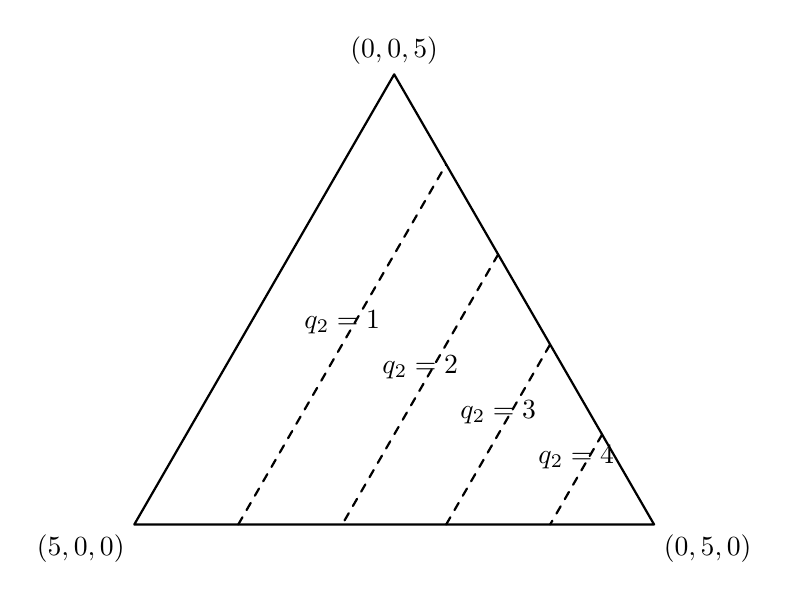
\begin{tikzpicture}[scale=1.1, line cap=round, line join=round]
  \pgfmathsetmacro{\N}{5} % sum of coordinates
  \pgfmathsetmacro{\S}{6} % side length (visual)

  % Equilateral triangle vertices
  \coordinate (A) at (0,0);                 % (N,0,0) i.e. q1=N
  \coordinate (B) at (\S,0);                % (0,N,0) i.e. q2=N
  \coordinate (C) at ({\S/2},{\S*sqrt(3)/2}); % (0,0,N) i.e. q3=N

  % Barycentric placement helper:
  % point with (q1,q2,q3) and q1+q2+q3 = N is
  % (q1/N)*A + (q2/N)*B + (q3/N)*C
  \newcommand{\Bary}[4]{%
    \pgfmathsetmacro{\wone}{#1/\N}%
    \pgfmathsetmacro{\wtwo}{#2/\N}%
    \pgfmathsetmacro{\wthree}{#3/\N}%
    \coordinate (#4) at ($ \wone*(A) + \wtwo*(B) + \wthree*(C) $);%
  }

  % Draw the simplex boundary
  \draw[thick] (A) -- (B) -- (C) -- cycle;

  % Label vertices
  \node[below left]  at (A) {$(5,0,0)$};
  \node[below right] at (B) {$(0,5,0)$};
  \node[above]       at (C) {$(0,0,5)$};

  % (Optional) label axes directions on edges
  % \node[font=\small, below] at ($(A)!0.5!(B)$) {$q_3=0$};
  % \node[font=\small, left]  at ($(A)!0.5!(C)$) {$q_2=0$};
  % \node[font=\small, right] at ($(B)!0.5!(C)$) {$q_1=0$};

  % Boundary for q1 - q3 = 1 intersects at (1,4,0) and (3,0,2)
  \Bary{4}{1}{0}{P} % (4,1,0)
  \Bary{0}{1}{4}{Q} % (0,1,4)
  \Bary{0}{2}{3}{S} % (3,2,0)
  \Bary{3}{2}{0}{T}
  \Bary{2}{3}{0}{R} % (0,2,3)
  \Bary{0}{3}{2}{L} % (2,3,0)
  \Bary{1}{4}{0}{N} % (0,3,2)
  \Bary{0}{4}{1}{M} % (1,4,0)
  \Bary{2}{2}{1}{X} % (2,2,1)
  \Bary{1.5}{1.5}{2}{Y}

  % % Shade region q1 - q3 > 1 (the side containing A=(5,0,0))
  % \fill[gray!25, opacity=0.7] (A) -- (Q) -- (P) -- cycle;
  % \fill[gray!25, opacity=0.7] (B) -- (S) -- (T) -- cycle;

  % Draw the boundary line (dashed since strict inequality)
  \draw[thick, dashed] (P) -- (Q) node[midway, above] {$q_2 = 1$};
  \draw[thick, dashed] (S) -- (T) node[midway, above] {$q_2 = 2$};
  \draw[thick, dashed] (R) -- (L) node[midway, above] {$q_2 = 3$};
  \draw[thick, dashed] (M) -- (N) node[midway, above] {$q_2 = 4$};

  % % Optional point labels
  % \fill (X) circle (1.2pt) node[above left, font=\small] {$(2,2,1)$};
  % \fill (Y) circle (1.2pt) node[below right, font=\small] {$(2.5,1.5,1)$};

  % Optional annotation
  % \node[font=\small] at ($(A)!0.35!(C)$) {$q_1-q_3>1$};
\end{tikzpicture}





\end{document}